\chapter{Аналитическая часть}

\section{Постановка задачи}

В рамках выполнения курсовой работы необходимо разработать загружаемый модуль ядра для мониторинга использования SLAB-кэша процессами в операционной системе Linux.
Для реализации поставленной задачи необходимо:
\begin{itemize}
	\item провести анализ распределителей памяти SLAB и SLUB;
	\item провести анализ и выбор механизмов перехвата функций;
	\item провести анализ методов передачи информации из пространства пользователя в пространство ядра и наоборот;
	\item разработать структуры и алгоритмы загржаемого модуля ядра;
	\item реализовать загружаемый модуль ядра для мониторинга использования SLAB-кэша процессами в операционной системе Linux;
	\item провести анализ работы реализованного загружаемого модуля ядра.
\end{itemize}

К разрабатываемому модулю ядра предъявляются следующие требования:
\begin{itemize}
	\item обеспечение передачи данных из пространства пользователя в пространство ядра и наоборот;
	\item возможность взаимодействия процессов из пространства пользователя с разработанным загружаемым модулем ядра;
	\item обеспечения сбора статистики использования SLAB-кэша для одного и более процессов;
	\item получение и хранение информации о SLAB-кэшах~--- PID процесса, имя кэша, число выделенных объектов, размер объекта, число объектов в одном slab, число страниц в одном slab, общее число выделенных страниц.
\end{itemize}

\section{Анализ распределителей памяти SLAB и SLUB}

Для многих структур, используемых в ядре, время, необходимое для инициализации объекта, превышает время, затрачиваемое на выделение для него памяти~\cite{slab_info}.
Для решения данной проблемы был разработан распределитель SLAB, основная идея которого заключается в хранении часто используемых объектов в инициализированном состоянии, доступном для использования ядром~\cite{slab_info}.

Взаимосвязь между составляющими распределителя SLAB представлена на рисунке~\ref{slab_relations}.
\begin{figure}[H]
	\centering
	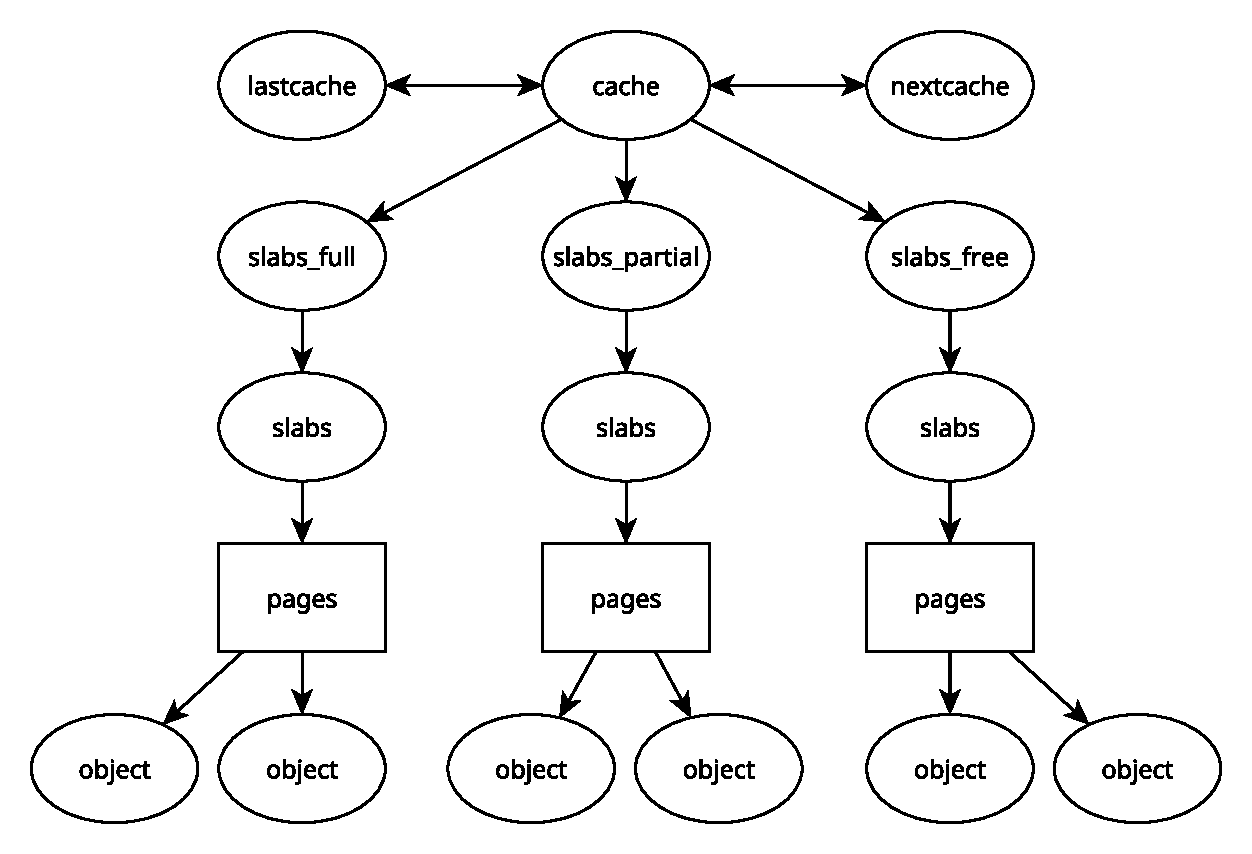
\includegraphics[width=0.8\linewidth]{slab_relations}
	\caption{Схема распределителя SLAB}
	\label{slab_relations}
\end{figure}

Распределитель SLAB состоит из переменного количества кэшей, которые содержатся в двусвязном циклическом списке~\cite{slab_info}.
Каждый кэш хранит в памяти блоки смежных страниц, которые разделены на небольшие фрагменты для хранения структур данных и объектов, которыми он управляет~\cite{slab_info}.
Существуют три вида фрагментов SLAB~\cite{slab_info}:
\begin{itemize}
	\item slabs\_full (полностью распределенные фрагменты);
	\item slabs\_partial (частично распределенные фрагменты);
	\item slabs\_empty (пустые фрагменты, не выделенные под объекты).
\end{itemize}

Поскольку объекты выделяются и освобождаются, отдельные фрагменты SLAB могут перемещаться между соответствующими списками~\cite{slab_info}.
Когда все объекты фрагмента SLAB израсходованы, система переносит их из списка slabs\_partial в список slabs\_full~\cite{slab_info}.
Когда фрагмент SLAB полон, и объект освобождается, он перемещается из списка slabs\_full в список slabs\_partial~\cite{slab_info}.
Когда освобождаются все объекты фрагмента, они перемещаются в список slabs\_empty~\cite{slab_info}.

Начиная с версии 2.6.23 ядра Linux используется SLUB~--- усовершенствованный распределитель SLAB~\cite{slub_info}.
В нем используется базовая модель SLAB, однако исправлены некоторые недостатки, особенно для систем с большим количеством процессоров~\cite{slub_info}.

\section{Анализ API для работы с распределителями SLAB и SLUB}

Основной структурой для работой с распределителями SLAB и SLUB ялвляется struct kmem\_cache, содержащий информацию о кэше. Объявление структуры struct~kmem\_cache для распределителя SLAB для ядра Linux версии 6.5.13 представлено в листинге~\ref{kmem_cache_slab}.
%\begin{figure}[H]
	\begin{lstlisting}[label=kmem_cache_slab,caption=Объявление структуры struct~kmem\_cache для распределителя SLAB (версия ядра Linux~--- 6.5.13),language=Caml]
struct kmem_cache{
	struct array_cache __percpu *cpu_cache;
	
	/* 1) Cache tunables. Protected by slab_mutex */
	unsigned int batchcount;
	unsigned int limit;
	unsigned int shared;
	
	unsigned int size;
	struct reciprocal_value reciprocal_buffer_size;
	/* 2) touched by every alloc & free from the backend */
	
	slab_flags_t flags;		/* constant flags */
	unsigned int num;		/* # of objs per slab */
	
	/* 3) cache_grow/shrink */
	/* order of pgs per slab (2^n) */
	unsigned int gfporder;
	
	/* force GFP flags, e.g. GFP_DMA */
	gfp_t allocflags;
	
	size_t colour;			/* cache colouring range */
	unsigned int colour_off;	/* colour offset */
	unsigned int freelist_size;
	
	/* constructor func */
	void ( *ctor)(void *obj);
	
	/* 4) cache creation/removal */
	const char *name;
	struct list_head list;
	int refcount;
	int object_size;
	int align;
	
	/* 5) statistics */
	#ifdef CONFIG_DEBUG_SLAB
	unsigned long num_active;
	unsigned long num_allocations;
	unsigned long high_mark;
	unsigned long grown;
	unsigned long reaped;
	unsigned long errors;
	unsigned long max_freeable;
	unsigned long node_allocs;
	unsigned long node_frees;
	unsigned long node_overflow;
	atomic_t allochit;
	atomic_t allocmiss;
	atomic_t freehit;
	atomic_t freemiss;
	
	/*
	* If debugging is enabled, then the allocator can add additional
	* fields and/or padding to every object. 'size' contains the total
	* object size including these internal fields, while 'obj_offset'
	* and 'object_size' contain the offset to the user object and its
	* size.
	*/
	int obj_offset;
	#endif /* CONFIG_DEBUG_SLAB */
	
	#ifdef CONFIG_KASAN_GENERIC
	struct kasan_cache kasan_info;
	#endif
	
	#ifdef CONFIG_SLAB_FREELIST_RANDOM
	unsigned int *random_seq;
	#endif
	
	#ifdef CONFIG_HARDENED_USERCOPY
	unsigned int useroffset;	/* Usercopy region offset */
	unsigned int usersize;		/* Usercopy region size */
	#endif
	
	struct kmem_cache_node *node[MAX_NUMNODES];
};
	\end{lstlisting}
%\end{figure}

Объявление структуры struct~kmem\_cache для распределителя SLAB для ядра Linux версии 6.5.13 представлено в листинге~\ref{kmem_cache_slub}.
%\begin{figure}[H]
	\begin{lstlisting}[label=kmem_cache_slub,caption=Объявление структуры struct~kmem\_cache для распределителя SLUB (версия ядра Linux~--- 6.5.13),language=Caml]
struct kmem_cache{
	#ifndef CONFIG_SLUB_TINY
	struct kmem_cache_cpu __percpu *cpu_slab;
	#endif
	/* Used for retrieving partial slabs, etc. */
	slab_flags_t flags;
	unsigned long min_partial;
	unsigned int size;	/* The size of an object including metadata */
	unsigned int object_size;/* The size of an object without metadata */
	struct reciprocal_value reciprocal_size;
	unsigned int offset;	/* Free pointer offset */
	#ifdef CONFIG_SLUB_CPU_PARTIAL
	/* Number of per cpu partial objects to keep around */
	unsigned int cpu_partial;
	/* Number of per cpu partial slabs to keep around */
	unsigned int cpu_partial_slabs;
	#endif
	struct kmem_cache_order_objects oo;
	
	/* Allocation and freeing of slabs */
	struct kmem_cache_order_objects min;
	gfp_t allocflags;	/* gfp flags to use on each alloc */
	int refcount;		/* Refcount for slab cache destroy */
	void ( *ctor)(void *);
	unsigned int inuse;		/* Offset to metadata */
	unsigned int align;		/* Alignment */
	unsigned int red_left_pad;	/* Left redzone padding size */
	const char *name;	/* Name (only for display!) */
	struct list_head list;	/* List of slab caches */
	#ifdef CONFIG_SYSFS
	struct kobject kobj;	/* For sysfs */
	#endif
	#ifdef CONFIG_SLAB_FREELIST_HARDENED
	unsigned long random;
	#endif
	
	#ifdef CONFIG_NUMA
	/*
	* Defragmentation by allocating from a remote node.
	*/
	unsigned int remote_node_defrag_ratio;
	#endif
	
	#ifdef CONFIG_SLAB_FREELIST_RANDOM
	unsigned int *random_seq;
	#endif
	
	#ifdef CONFIG_KASAN_GENERIC
	struct kasan_cache kasan_info;
	#endif
	
	#ifdef CONFIG_HARDENED_USERCOPY
	unsigned int useroffset;	/* Usercopy region offset */
	unsigned int usersize;		/* Usercopy region size */
	#endif
	
	struct kmem_cache_node *node[MAX_NUMNODES];
};
	\end{lstlisting}
%\end{figure}

Для создания нового SLAB-кэша применяется функция kmem\_cache\_create~\cite{slab_info}, прототип которой представлен в листинге~\ref{kmem_cache_create}.
\begin{figure}[H]
	\begin{lstlisting}[label=kmem_cache_create,caption=Прототип функции kmem\_cache\_create (версия ядра Linux~--- 6.5.13),language=Caml]
struct kmem_cache *kmem_cache_create(
	const char *name,       /* имя кэша */
	unsigned int size,      /* размер выделяемых в кэше объектов */
	unsigned int align,     /* выравнивание объектов */
	slab_flags_t flags,     /* флаги SLAB */
	void ( *ctor)(void *)   /* конструктор выделяемых в кэше объектов */
);
	\end{lstlisting}
\end{figure}

Существуют следующие флаги SLAB~\cite{mm_api}:
\begin{itemize}
	\item SLAB\_POISON~--- запись в SLAB шаблонного значения 0x5a5a5a5a (используется для получения ссылок на неинициализированную память);
	\item SLAB\_RED\_ZONE~--- вставка <<красных зон>> в выделенные участки памяти для отслеживания переполнения;
	\item SLAB\_HWCACHE\_ALIGN~--- выделение объектов в кэше по аппаратной линии кэширования.
\end{itemize}

Для уничтожения SLAB-кэша применяется системный вызов kmem\_cache\_destroy~\cite{slab_info}.
Прототип функции kmem\_cache\_destroy представлен в листинге~\ref{kmem_cache_destroy}.
Диаграмма вызовов для функции kmem\_cache\_destroy представлена на рисунке~\ref{kmem_cache_destroy_call_diag}.
\begin{figure}[H]
	\begin{lstlisting}[label=kmem_cache_destroy,caption=Прототип функции kmem\_cache\_create (версия ядра Linux~--- 6.5.13),language=Caml]
void kmem_cache_destroy(
	struct kmem_cache *s  /* указатель на SLAB-кэш */
);
	\end{lstlisting}
\end{figure}
\begin{figure}[H]
	\centering
	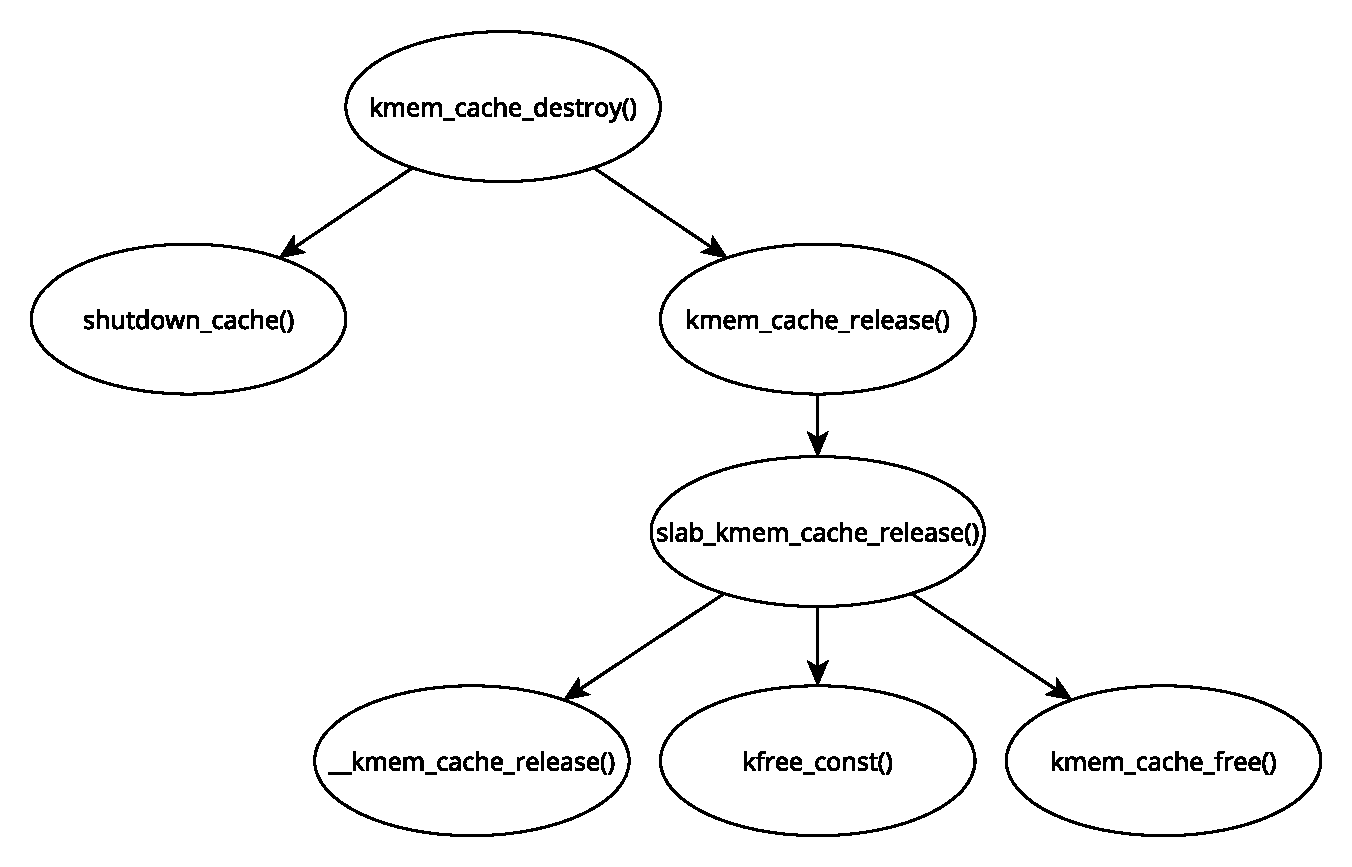
\includegraphics[width=0.9\linewidth]{kmem_cache_destroy_call_diag}
	\caption{Диаграмма вызовов для функции kmem\_cache\_destroy (версия ядра Linux~--- 6.5.13)}
	\label{kmem_cache_destroy_call_diag}
\end{figure}

Для выделения памяти из SLAB-кэша применяются системные вызовы kmem\_cache\_alloc и kmalloc~\cite{slab_info}.
Прототипы функций kmem\_cache\_alloc и kmalloc представлены в листингах~\ref{kmem_cache_alloc} и \ref{kmalloc} соответственно.
\begin{figure}[H]
	\begin{lstlisting}[label=kmem_cache_alloc,caption=Прототип функции kmem\_cache\_alloc (версия ядра Linux~--- 6.5.13),language=Caml]
void *kmem_cache_alloc(
	struct kmem_cache *cachep,  /* указатель на SLAB-кэш */
	gfp_t flags                 /* флаги GFP, определяющие поведение
	                               при выделении памяти */
);
	\end{lstlisting}
\end{figure}
\begin{figure}[H]
	\begin{lstlisting}[label=kmalloc,caption=Прототип функции kmalloc (версия ядра Linux~--- 6.5.13),language=Caml]
void *kmalloc(
	size_t size,  /* размер выделяемого объекта */
	gfp_t flags   /* флаги GFP, определяющие поведение
	                 при выделении памяти */
);
	\end{lstlisting}
\end{figure}

Существуют следующие GFP-флаги~\cite{gfp}:
\begin{itemize}
	\item GFP\_ATOMIC~--- процесс не может уснуть во время выделения памяти;
	\item GFP\_NOIO~--- запрет на операции ввода/вывода во время выделения памяти;
	\item GFP\_NOHIGHIO~--- используется системным вызовом alloc\_bounce\_page() во время создания буфера отказов для ввода-вывода в верхней памяти;
	\item GFP\_NOFS~--- используется только буферным кэшем и файловыми системами для избежания рекурсии;
	\item GFP\_KERNEL~--- выделение памяти от имени процесса в пространстве ядра;
	\item GFP\_USER~--- выделение памяти от имени процесса в пространстве пользователя;
	\item GFP\_HIGHUSER~--- выделение страниц из верхней памяти от имени пользователя.
\end{itemize}

На рисунках~\ref{kmem_cache_alloc_call_diag}~и~\ref{kmalloc_call_diag} представлены диаграммы вызовов для функций kmem\_cache\_alloc и kmalloc соответственно.
\begin{figure}[H]
	\centering
	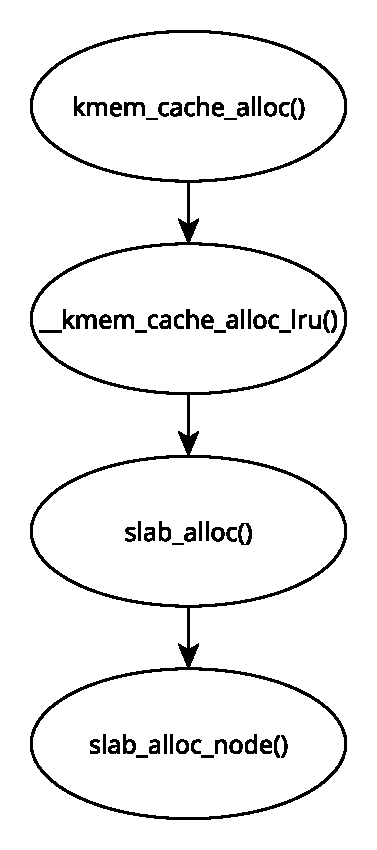
\includegraphics[width=0.25\linewidth]{kmem_cache_alloc_call_diag}
	\caption{Диаграмма вызовов для функции kmem\_cache\_alloc (версия ядра Linux~--- 6.5.13)}
	\label{kmem_cache_alloc_call_diag}
\end{figure}
\begin{figure}[H]
	\centering
	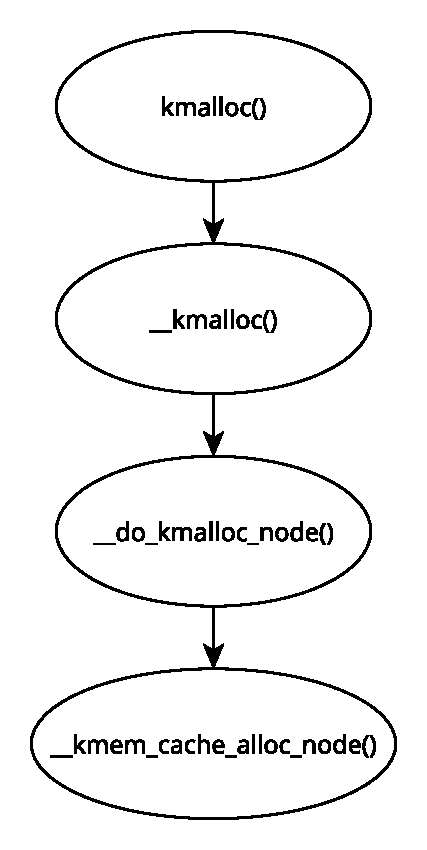
\includegraphics[width=0.25\linewidth]{kmalloc_call_diag}
	\caption{Диаграмма вызовов для функции kmalloc (версия ядра Linux~--- 6.5.13)}
	\label{kmalloc_call_diag}
\end{figure}

В отличие от kmem\_cache\_alloc, функция kmalloc не принимает в качестве параметра указатель на объект структуры struct~kmem\_cache.
Системный вызов kmalloc осуществляет поиск кэша, который соответствует указанному размеру, и передает в качестве параметра указатель на него функции \_\_kmem\_cache\_alloc\_node для последующего выделения памяти.

Для освобождения выделенной из SLAB-кэша памяти используются системные вызовы kmem\_cache\_free и kfree~\cite{slab_info}.
Прототипы функций kmem\_cache\_free и kfree представлены в листингах~\ref{kmem_cache_free} и \ref{kfree} соответственно.
\begin{figure}[H]
	\begin{lstlisting}[label=kmem_cache_free,caption=Прототип функции kmem\_cache\_free (версия ядра Linux~--- 6.5.13),language=Caml]
void kmem_cache_free(
	struct kmem_cache *s,  /* указатель на SLAB-кэш */
	void *objp             /* указатель на освобождаемый объект */
);
	\end{lstlisting}
\end{figure}
\begin{figure}[H]
	\begin{lstlisting}[label=kfree,caption=Прототип функции kfree (версия ядра Linux~--- 6.5.13),language=Caml]
void kfree(
	const void *objp  /* указатель на освобождаемый объект */
);
	\end{lstlisting}
\end{figure}

На рисунках~\ref{kmem_cache_free_call_diag}~и~\ref{kfree_call_diag} представлены диаграммы вызовов для функций kmem\_cache\_free и kfree соответственно.
\begin{figure}[H]
	\centering
	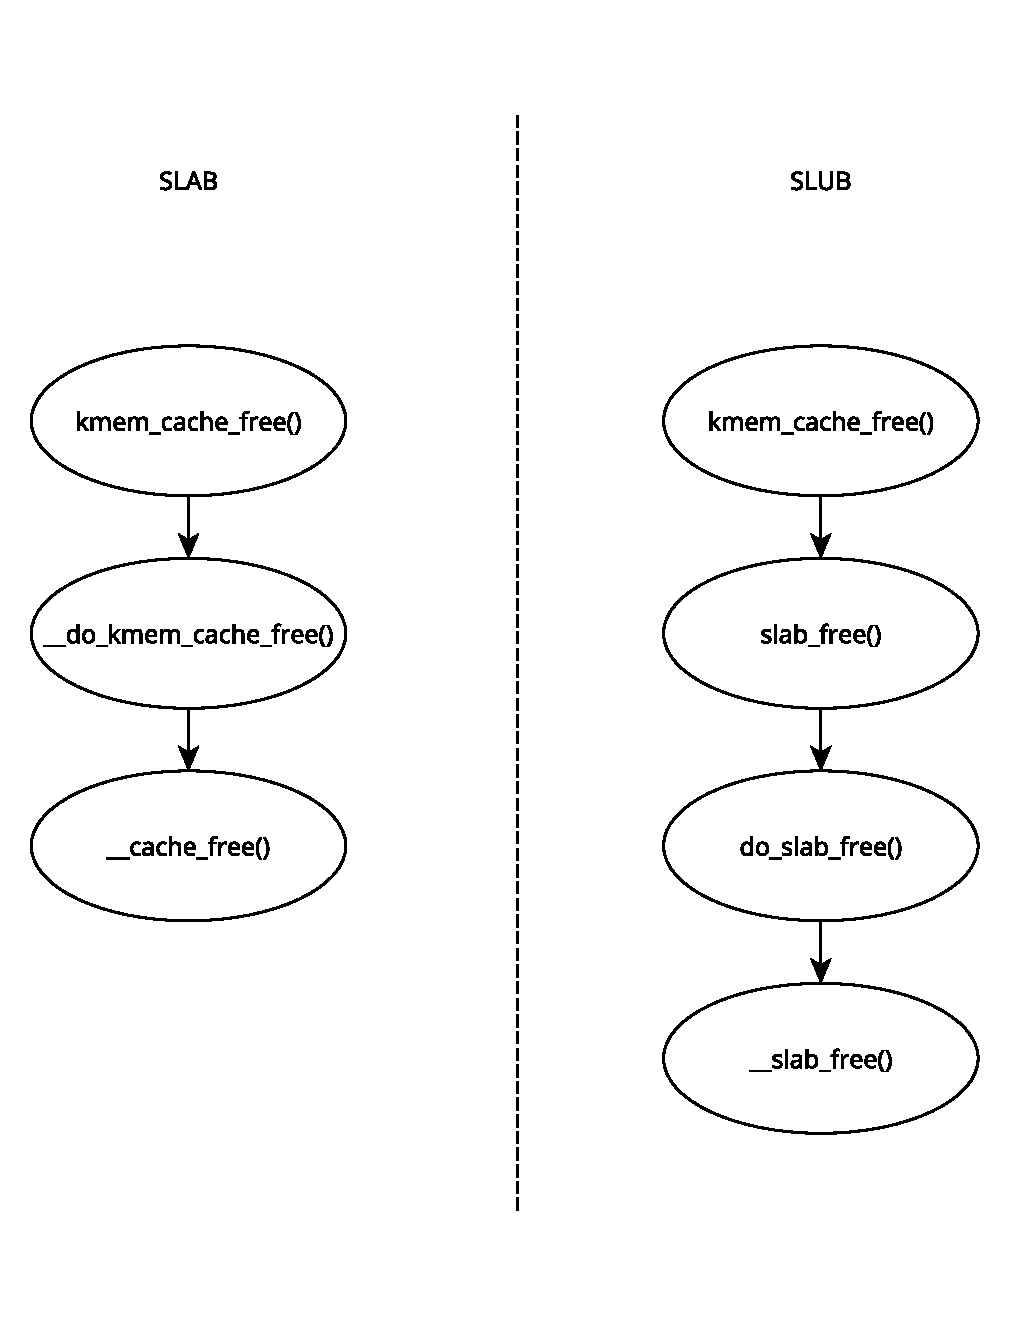
\includegraphics[width=0.45\linewidth]{kmem_cache_free_call_diag}
	\caption{Диаграмма вызовов для функции kmem\_cache\_free (версия ядра Linux~--- 6.5.13)}
	\label{kmem_cache_free_call_diag}
\end{figure}
\begin{figure}[H]
	\centering
	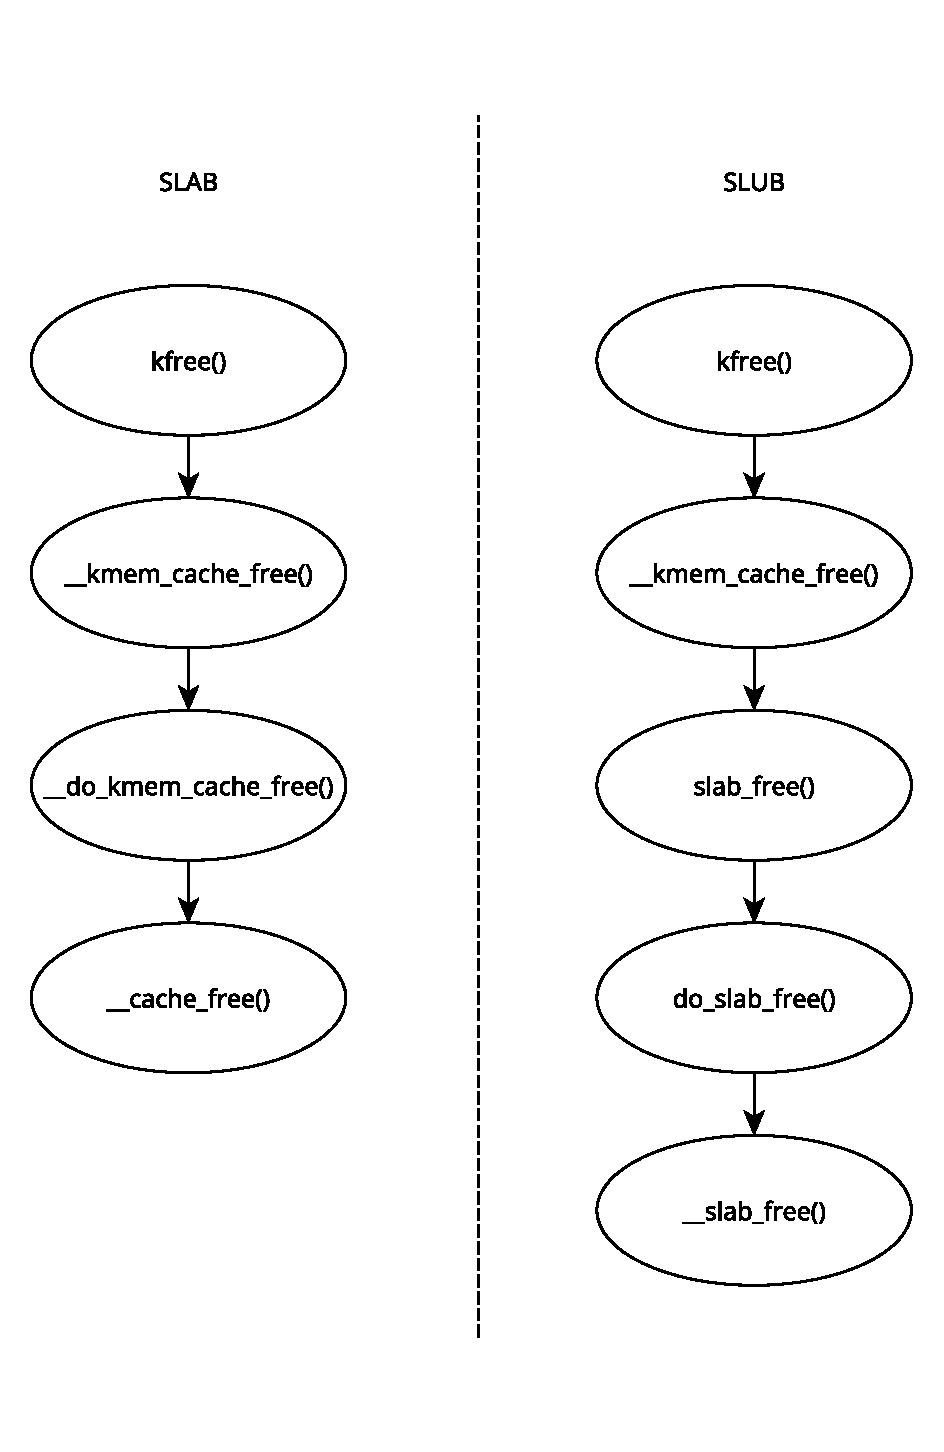
\includegraphics[width=0.45\linewidth]{kfree_call_diag}
	\caption{Диаграмма вызовов для функции kfree (версия ядра Linux~--- 6.5.13)}
	\label{kfree_call_diag}
\end{figure}

Системный вызов kfree осуществляет поиск кэша, из которого был выделен объект, и передает в качестве параметра указатель на него функции \_\_kmem\_cache\_free для последующего освобождения объекта.

Таким образом, для сбора информации об использовании SLAB-кэша необходимо оосуществить перехват следующих функций:
\begin{itemize}
	\item \_\_kmem\_cache\_alloc\_node,
	\item \_\_kmem\_cache\_free,
	\item kmem\_cache\_alloc,
	\item kmem\_cache\_free,
	\item kmem\_cache\_destroy.
\end{itemize}

\section{Механизмы перехвата функций}

Идея перехвата функции заключается в изменении некоторого адреса в памяти процесса или кода в теле функции так, чтобы при вызове перехватываемой функции управление передавалось подменяемой функции.
Данная функция выполняется вместо системной функции, производя необходимые действия до и после вызова оригинальной функции.

В данной работе перехват функций необходим для получения статистики использования SLAB-кэшей и и информации о них, поскольку структура struct~kmem\_cache не содержит информацию о процессах, использующих данный кэш.

Существуют следующие наиболее известные подходы перехвата функций: kprobes~\cite{kprobes} и ftrace~\cite{ftrace}.

\subsection{kprobes}

kprobes представляет собой специальный интерфейс, предназначенный для отладки и трассировки ядра~\cite{kprobes}.
Данный интерфейс позволяет устанавливать пред- и постобработчики для любой инструкции в ядре, а так же обработчики на вход и возврат из функции~\cite{kprobes}.
Обработчики получают доступ к регистрам и могут изменять их значение, что позволяет использовать kprobes как в целях мониторинга, так и для влияния на дальнейшую работу ядра~\cite{kprobes}.

Интерфейс kprobes имеет следующие особенности~\cite{kprobes}:
\begin{itemize}
	\item перехват любой инструкции в ядре реализуется с помощью точек останова, внедряемых в исполняемый код ядра;
	\item относительно большие накладные расходы (для расстановки и обработки точек останова необходимо большое количество процессорного времени);
	\item техническая сложность реализации (в частности, чтобы получить аргументы функции или значения её локальных переменных, нужно извлекать их из регистров или стека).
\end{itemize}

\subsection{ftrace}

ftrace~--- фреймворк для трассировки ядра на уровне функций, реализованный на основе ключей компилятора pg и mfentry~\cite{ftrace_com}.
Данные функции вставляют в начало каждой функции вызов специальной трассировочной функции mcount() или \_\_fentry\_\_()~\cite{ftrace_com}.
В пользовательских программах данная возможность компилятора используется профилировщиками, целью отслеживания всех вызываемых функций~\cite{ftrace_com}.
В ядре эти функции используются исключительно для реализации рассматриваемого фреймворка~\cite{ftrace_com}.

Для большинства современных архитектур процессора доступна оптимизация~--- динамический frace~\cite{ftrace_com}.
Ядро знает расположение всех вызовов функций mcount() или \_\_fentry\_\_() и на ранних этапах загрузки ядра подменяет их машинный код на специальную машинную инструкцию NOP [8], которая ничего не делает~\cite{ftrace_com}.
При включении трассировки, в нужные функции необходимые вызовы добавляются обратно.
Если ftrace не используется, его влияние на производительность системы минимально.

Фреймворк ftrace имеет следующие особенности~\cite{ftrace_com}:
\begin{itemize}
	\item возможность перехвата любой функции;
	\item совместимость перехвата функции с трассировкой;
	\item фреймворк зависит от конфигурации ядра, при этом в популярных конфигурациях ядра установлены все необходимые флаги для работы.
\end{itemize}

Для регистрации callback-функции необходима структура struct~ftrace\_ops~\cite{ftrace}.
Эта структура используется, чтобы сообщить ftrace, какая callback-функция должна вызываться, а также какая защита будет выполнятся обратным вызовом и не потребует обработки ftrace~\cite{ftrace}.
Объявление структуры struct~ftrace\_ops представлено в листинге~\ref{struct_ftrace_ops}.
\begin{figure}[H]
	\begin{lstlisting}[label=struct_ftrace_ops,caption=Объявление структуры struct~ftrace\_ops (версия ядра Linux~--- 6.5.13),language=Caml]
struct ftrace_ops{
	ftrace_func_t func;
	struct ftrace_ops __rcu *next;
	unsigned long flags;
	void *private;
	ftrace_func_t saved_func;
	#ifdef CONFIG_DYNAMIC_FTRACE
	struct ftrace_ops_hash local_hash;
	struct ftrace_ops_hash *func_hash;
	struct ftrace_ops_hash old_hash;
	unsigned long trampoline;
	unsigned long trampoline_size;
	struct list_head list;
	ftrace_ops_func_t ops_func;
	#ifdef CONFIG_DYNAMIC_FTRACE_WITH_DIRECT_CALLS
	unsigned long direct_call;
	#endif
	#endif
};
	\end{lstlisting}
\end{figure}

Для регистрации callback-функции необходимо определить поле func объекта структуры struct~ftrace\_ops и вызвать функцию register\_ftrace\_function~\cite{ftrace}.
Для дерегистрации callback-функции необходимо применить системный вызов unregister\_ftrace\_function~\cite{ftrace}.
Прототипы функций register\_ftrace\_function и unregister\_ftrace\_function представлены в листингах~\ref{register_ftrace_function}~и~\ref{unregister_ftrace_function} соотвественно.
\begin{figure}[H]
	\begin{lstlisting}[label=register_ftrace_function,caption=Прототип функции register\_ftrace\_function (версия ядра Linux~--- 6.5.13),language=Caml]
int register_ftrace_function(
	struct ftrace_ops *ops
);
	\end{lstlisting}
\end{figure}
\begin{figure}[H]
	\begin{lstlisting}[label=unregister_ftrace_function,caption=Прототип функции unregister\_ftrace\_function (версия ядра Linux~--- 6.5.13),language=Caml]
int unregister_ftrace_function(
	struct ftrace_ops *ops
);
	\end{lstlisting}
\end{figure}

Callback-функция должна иметь прототип, представленный в листинге~\ref{ftrace_callback_proto}.
\begin{figure}[H]
	\begin{lstlisting}[label=ftrace_callback_proto,caption=Прототип callback-функции для работы с ftrace,language=Caml]
void callback_func(
	unsigned long ip,         /* указатель на отслеживаемую функцию */
	unsigned long parent_ip,  /* указатель на функцию, вызвавшая
	                             отслеживаемую функцию */
	struct ftrace_ops *op,
	struct pt_regs *regs      /* указатель на объект структуры,
	                             позволяющего установить значения
	                             в регистрах процессора после
	                             выхода из callback функции,
	                             если был установлен соответствующий
	                             флаг */
);
	\end{lstlisting}
\end{figure}

Для перехвата функции необходимо в callback-функции изменить поле ip объекта regs структуры struct~pt\_regs на адрес новой функции.

\section{Виртуальная файловая система proc}

Виртуальная файловая система proc~--- специальный интерфейс, с помощью которого можно мгновенно получить некоторую информацию о ядре в пространстве пользователя и передать информацию в пространство ядра~\cite{proc}.

Директория /proc содержит, в частности, по одному подкаталогу для каждого запущенного в системе процесса~\cite{proc}.
Имя каждого такого подкаталога является числом, значение которого равно PID соответствующего процесса~\cite{proc}.
Помимо информации о каждом запущенном процессе виртуальная файловая система proc предоставляет данные о работе ядра системы~\cite{proc}.

Для работы с файлами в виртуальной файловой системе proc используется структура struct~proc\_ops, содержащая указатели на функции взаимодействия с файлом, такие как открытие, закрытие, чтение и запись.
Объявление структуры struct~proc\_ops представлено в листинге~\ref{struct_proc_ops}.
\begin{figure}[H]
	\begin{lstlisting}[label=struct_proc_ops,caption=Объявление структуры struct~proc\_ops (версия ядра Linux~--- 6.5.13),language=Caml]
struct proc_ops
{
	unsigned int proc_flags;
	int	( *proc_open)(struct inode *, struct file *);
	ssize_t	( *proc_read)(struct file *, char __user *, size_t, loff_t *);
	ssize_t ( *proc_read_iter)(struct kiocb *, struct iov_iter *);
	ssize_t	( *proc_write)(struct file *, const char __user *, size_t, loff_t *);
	/* mandatory unless nonseekable_open() or equivalent is used */
	loff_t	( *proc_lseek)(struct file *, loff_t, int);
	int	( *proc_release)(struct inode *, struct file *);
	__poll_t ( *proc_poll)(struct file *, struct poll_table_struct *);
	long	( *proc_ioctl)(struct file *, unsigned int, unsigned long);
	#ifdef CONFIG_COMPAT
	long	( *proc_compat_ioctl)(struct file *, unsigned int, unsigned long);
	#endif
	int	( *proc_mmap)(struct file *, struct vm_area_struct *);
	unsigned long ( *proc_get_unmapped_area)(struct file *, unsigned long, unsigned long, unsigned long, unsigned long);
} __randomize_layout;
	\end{lstlisting}
\end{figure}

Для создания файла в виртуальной файловой системе proc используется системный вызов proc\_create, прототип которого представлен в листинге~\ref{proc_create}.
\begin{figure}[H]
	\begin{lstlisting}[label=proc_create,caption=Прототип функции proc\_create (версия ядра Linux~--- 6.5.13),language=Caml]
struct proc_dir_entry *proc_create(
	const char *name,                 /* имя файла */
	umode_t mode,                     /* флаги, описывающие разрешения
	                                     на чтение и запись */
	struct proc_dir_entry *parent,    /* указатель на объект структуры
	                                     proc_dir_entry, описывающий
	                                     родительскую директорию
	                                     ( если parent равно NULL, то файл
	                                     создаётся в директории /proc) */
	const struct proc_ops *proc_ops   /* указатель на объект структуры
	                                     proc_ops, содержащий
	                                     указатели на функции
	                                     работы с файлом */
);
	\end{lstlisting}
\end{figure}

Функция proc\_create возвращает указатель на объект структуры proc\_dir\_entry созданного файла при успехе или NULL при неудаче.

\section{Взаимодействие процесса с загружаемым модулем ядра}

Для взаимодействия приложений с ядром и ядра с приложениями используются функции ядра copy\_to\_user и copy\_from\_user.

Функция copy\_to\_user копирует данные из пространства ядра в пространство пользователя.
Прототип функции copy\_to\_user представлен в листинге~\ref{copy_to_user}.
\begin{figure}[H]
	\begin{lstlisting}[label=copy_to_user,caption=Прототип функции copy\_to\_user (версия ядра Linux~--- 6.5.13),language=Caml]
long copy_to_user(
	void __user *to,   /* адрес буфера в пространстве пользователя */
	const void *from,  /* адрес буфера в пространстве ядра */
	long n             /* количество копируемых байт */
);
	\end{lstlisting}
\end{figure}

Функция copy\_to\_user возвращает количество байт, которые не могут быть скопированы.
В случае успешного выполнения будет возвращен 0.

Функция copy\_from\_user копирует данные из пространства пользователя в пространство ядра.
Прототип функции copy\_from\_user представлен в листинге~\ref{copy_from_user}.
\begin{figure}[H]
	\begin{lstlisting}[label=copy_from_user,caption=Прототип функции copy\_to\_user (версия ядра Linux~--- 6.5.13),language=Caml]
long copy_from_user(
	void __user *to,   /* адрес буфера в пространстве ядра */
	const void *from,  /* адрес буфера в пространстве пользователя */
	long n             /* количество копируемых байт */
);
	\end{lstlisting}
\end{figure}

Функция возвращает количество байт, которые не могут быть скопированы.
В случае успешного выполнения будет возвращен 0.

\section*{Вывод}

Была поставлена задача по разработке загружаемого модуля ядра для мониторинга использования SLAB-кэша процессами в операционной системе Linux.
Был проведен анализ распределителей SLAB и SLUB и API для работы с ними, механизмы перехвата функций kprobes и ftrace, виртуальной файловой системы proc.

Для перехвата функции был выбран фреймворк ftrace, поскольку он позволяет перехватит любую функцию по ее имени, загружается в ядро динамически и имеет задокументированный API.
